\documentclass[12pt]{article}
\usepackage{graphicx}
\usepackage[utf8]{inputenc}
\usepackage[greek, english]{babel}
\usepackage{alphabeta}
\usepackage{libertine}
%\usepackage{fancyhdr}
\usepackage[hidelinks]{hyperref}  % For hyperlinks without borders
\usepackage{hyperref}

\usepackage{geometry}

\usepackage{xcolor}

\usepackage{setspace}
\setstretch{1.5}  % Adjust the line spacing factor

\usepackage{titlesec}
\usepackage{titletoc}
% Adjust the space above and below \section titles
\titleformat{\section}{\normalfont\Large\bfseries}{\thesection}{1em}{}[\vspace{1ex}]
% Adjust the space between sections in the table of contents
\titlecontents{section}[0em]{\vspace{1ex}}{\thecontentslabel\hspace{1em}}{}{\titlerule*[1pc]{.}\contentspage}

\usepackage{caption}

\usepackage{wrapfig}


\geometry{
	left=0.5in,   % left margin
	right=0.5in,  % right margin
	top=0.6in,    % top margin
	bottom=0.6in  % bottom margin
}

\hypersetup{
	colorlinks=true,
	linkcolor=black,  % set the color for internal links
	urlcolor=blue    % set the color for external links
}

\DeclareCaptionLabelFormat{customlabel}{Εικόνα 3.1}
\captionsetup[figure]{labelformat=customlabel, labelsep=period}

\begin{document}
	
	\begin{titlepage}
		\centering
		
\includegraphics[width=0.5\textwidth]{photos/aueb_logo.jpg}
		\vfill
		\Huge\textbf{Your Title}
		\vspace{1cm}
		\Large\textbf{Your Subtitle}
		\vfill
		\today
	\end{titlepage}
	
	\renewcommand{\contentsname}{Περιεχόμενα}
	\tableofcontents
	
	\newpage  % Start content on a new page
	
	\section{Εισαγωγή}
	Το Youtube είναι ένας ιστότοπος κοινοποίησης, αποθήκευσης, αναζήτησης και αναπαραγωγής βίντεο. Κάθε χρήστης μπορεί να δημιουργήσει λογαριασμό και να ανεβάζει τα δικά του βίντεο ή ακόμα και να αναπαράγει σε πραγματικό χρόνο. Εκτός από τους χρήστες, πρόσβαση έχει ο οποιοσδήποτε στον ιστότοπο αυτό όπου μπορεί μόνο να παρακολουθεί τα βίντεο άλλων χρηστών. Το προφίλ του χρήστη παρουσιάζεται ως κανάλι όπου άλλοι χρήστες μπορούν να εγγραφούν ώστε να παρακολουθούν και να ενημερώνονται για βίντεο ή για πραγματικού χρόνου αναπαραγωγές που τους ενδιαφέρουν. Τα βίντεο που ανεβάζει ο κάθε χρήστης είναι συνηθως αποθηκευμένα σε playlists αναλόγως με την μορφή και το θέμα που έχουν. Επίσης στο κανάλι του ο κάθε χρήστης μπορεί να έχει κανάλια άλλων χρηστών που όπως αναφέρονται στην αγγλική ορολογία "Featured channels". Τα επιλεγμένα αυτα κανάλια αποτελούν κανάλια όπου ενας χρήστης επιλέγει να τα συμπεριλάβει στο δικο του κανάλι(δεν φαίνονται στο κοινό). Ο λόγος που γίνεται αυτό είναι για να προωθούν οι χρήστες και να εμφανίζουν άλλα κανάλια που τους αρέσουν, με τα οποία μπορεί να συνεργάζονται ή να θέλουν να τα προτείνους στους θεατές τους. Έτσι με αυτό τον τρόπο, οι χρήστες μπορούν να προσεγγίσουν πολλά είδη κοινού και να αυξήσουν ετσι τις εγγραφές και τις προβολές τους. Στην ανάλυση αυτή θα εξετάσουμε το κανάλι Samsung. Το κανάλι αυτό είναι το κανάλι του ομίλου εταιρειών Samsung που έχει ως σκοπό την ενημέρωση σχετικά με εκδηλώσεις, καινοτομες ταιχνολογίες, αφαρμογές και υπηρεσίες,  B2B solutions, παρουσιάσεις, και τις τελευταίες και καινοτόμες τεχνολογίες του ομίλου.
	\label{chap:intro_1}
	
	\section{Λήψη δεδομένων}
	Τα δεδομενα για την ανάλυση μας τα πήραμε με τη χρήση του \href{https://labs.polsys.net}{Bernhard Reiner's Tool} χρησιμοποιόντας τα YouTube Data Tools. Αρχικά, χρησιμοποιόντας το link του καναλιου στο YouTube, βρήκαμε το id του καναλιού μέσω του  \href{https://ytdt.digitalmethods.net/mod_channel_info.php}{Channel Info Module}. Έπειταμ με τη χρήση του \href{https://ytdt.digitalmethods.net/mod_channel_info.php}{Channel Network Module}, πήραμε δεδομένα για το δίκτυο του καναλιού. Οι παραμέτροι που χρησιμοποιήθηκαν ηταν το seed(αρχικό κανάλι) με τη χρηση του id με crawl depth ίσον με 2(το crawl depth καθορίζει πόσο βαθιά στο δίκτυο μπορουμε να φτάσουμε. Για παράδειγμα με depth=0 το εργαλείο αυτο επιστρέφει το δίκτυο με τις συσχετίσεις ανάμεσα στα seeds που δίνονται, με dept=1 επιστρέφει τα featured channels που έχει ο χρήστης στο κανάλι του και με depth=2 επιστρέφει τα featured channels που υπάρχουν στα κανάλια που βρήκαμε στο depth=1). Η επιλογή για της εγγραφές δεν λήφθηκε υπόψην δίοτι θέλαμε τα δεδομένα να είναι μόνο με τα featured channels. Μετά απο αυτά τα βήματα το εργαλείο δημιούργησς ενα gdf αρχείο το οποίο φορτώσαμε στο πρόγραμμα Gephi για ανάλυση. Εδω να σημεωθει οτι μέσω του Gephi έγινε έλεγχος των δεδομένων για τυχόν σφάλατα που θα μπορούσαν να επηρεάσουν την ανάλυση μας όπως για παρέδειγμα ο έλεγχος δυπλοτύπων, όπου σε μια περίπτωση υπήρκε διπλότυπο όπου και εντιμετωπίστηκε μέσω του Gephi, ο έλεγχος για null τιμές κ.α. \textcolor{red}{Σε μερικές περιπτώσεις υπήρχαν μη διαθέσιμες τιμές. Για παράδειγμα σε ορισμένους κόμβους, δεν υπήρχε στο αντίστοιχο κελί η χώρα ενώ ήταν γνωστή. Επομένως εισήχθησαν χοιροκίνητα οι τιμές όπου ηταν εφικτό. Σε άλλες περιπτώσεις, τυχόν σφάλματα αντιμετωπίζονται αναλόγως τη δεδομένη στιγμή όπου και αναφέρονται.}
	\label{chap:data_fetching_2}
	
	
	\section{Γραφική Αναπαράσταση Δικτύου}
	Το δίκτυο μόνο με τα ονόματα των κόμβων(καναλιών) χωρίς κάποια παραμετροποίηση.
		\begin{center}
			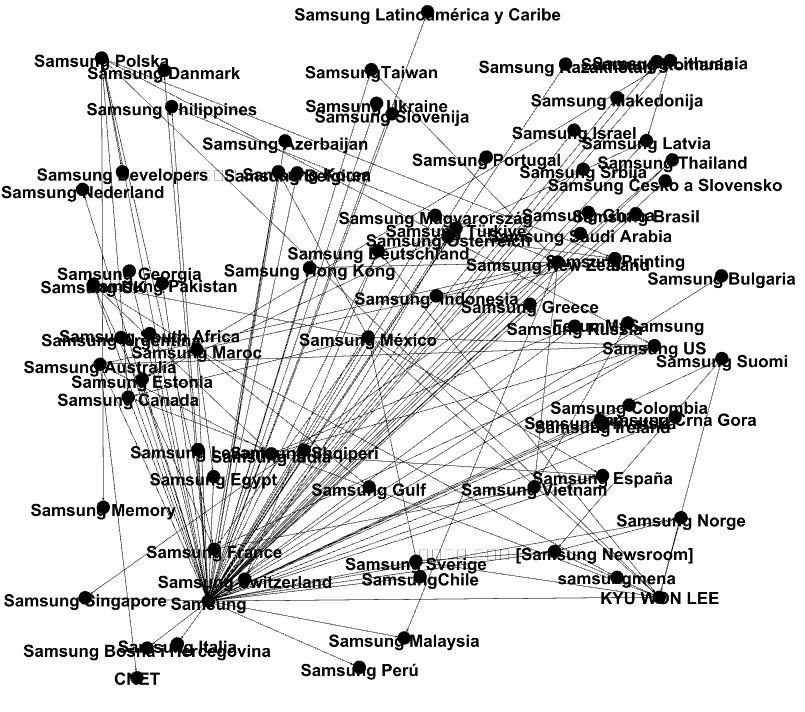
\includegraphics[width=0.7\textwidth]{photos/section3/first_painting.jpg}
		\end{center}
	\vspace{215pt}
	
	Επίσης μέσω του Gephi μπορούμε να θέσουμε διάφορες παραμέτρους όσον αφορά τoν χρωμaτισμό και την διάταξη ανάλογα με ορισμένες ιδιότητες που έχει το δίκτυο μας. Για παράδειγμα, για τη μορφή των κόμβων θέσαμε το μέγεθος του κάθε κόμβου ανάλογα με το πλήθος των εγγραφών(subscribercount) που έχει το κανάλι που αντιπροσοπεύει και για τον χρωματισμό θέσαμε ασπρο-πορτοκαλι-κοκκινο στο χαρακτηριστικο των προβολών(viewcount(100s)). Για την διάταξη, τρέξαμε τον Atlas Force 2 για να αραιώσουμε τον γράφο μας και τον Label Adjust για να διαχωριστουν οι ετικέτες ονομάτων των κόμβων. Έτσι προέκυψε η πάρακάτω εικόνα:
		\begin{center}
			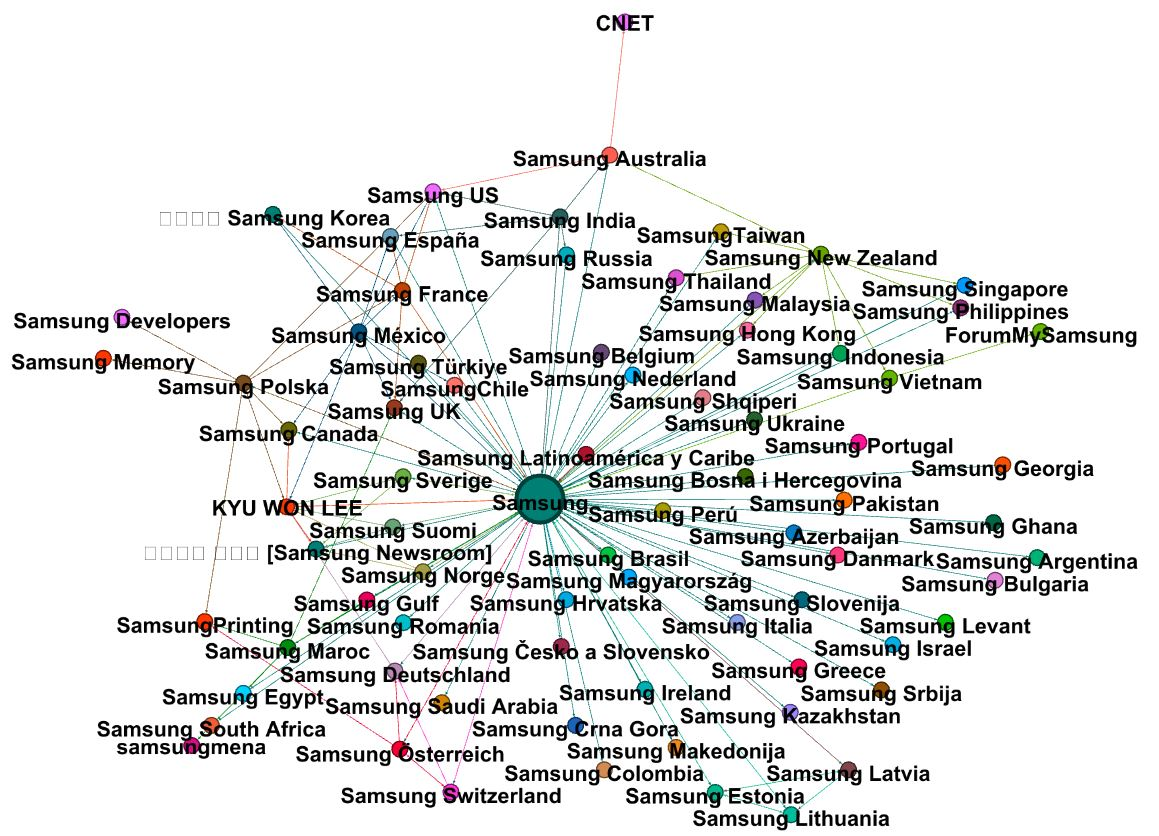
\includegraphics[width=0.8\textwidth]{photos/section3/second_painting.jpg}
		\end{center}
	Απο την εικόνα αυτή, τα δεδομένα που λαμβάνουμε είνα ο αριθμός των εγγραφών σε ενα κανάλι παίζει αρκετό ρόλο με τις προβολές που μπορεί να εχει, πραγμα αναμενόμενο για τον ιστότοπο που συζητάμε.
	\vspace{188pt}
	
	Βλέποντας τα δεδομένα του δικτύου μας απο το Data Laboratory του Gephi, παρατηρήσαμε πως υπάρχουν κανάλια απο διάφορες χώρες. Επομένως θεωρήσαμε ενδιαφέρον να κάνουμε μία παραμετροποίηση με τις χώρες ως εξής. Ο χρωματισμός έγινε μέσω διφορετικών χρωματων, τοσων, όσος και ο αριθμός των κόμβων μέσω του partition tab. Στο σημείο αυτο, θεώρήσαμε επίσης σημαντικό και την αναφορά του seed. Αυτό έγινε μεσω του μεγέθους των κόμβων μέσω του Ranking(αντίστοιχη μεταβλητη με την isseed εαν χρησιμοποιούσαμε τον χρωματισμό). Στη συνέχεια μέσω του Plugin Circular Layout που κατεβάσαμε μέσω των Tools του Gephi, δημιουργήσαμε την πιο κάτω διάταξη θέτοντας στην ιδιότητα "Order Nodes By" την χώρα. Για άλλη μια φορά, χρησιμοποιήσαμε τον Label Adjust για διαχωρισμό των ετοικετών.
		\begin{center}
			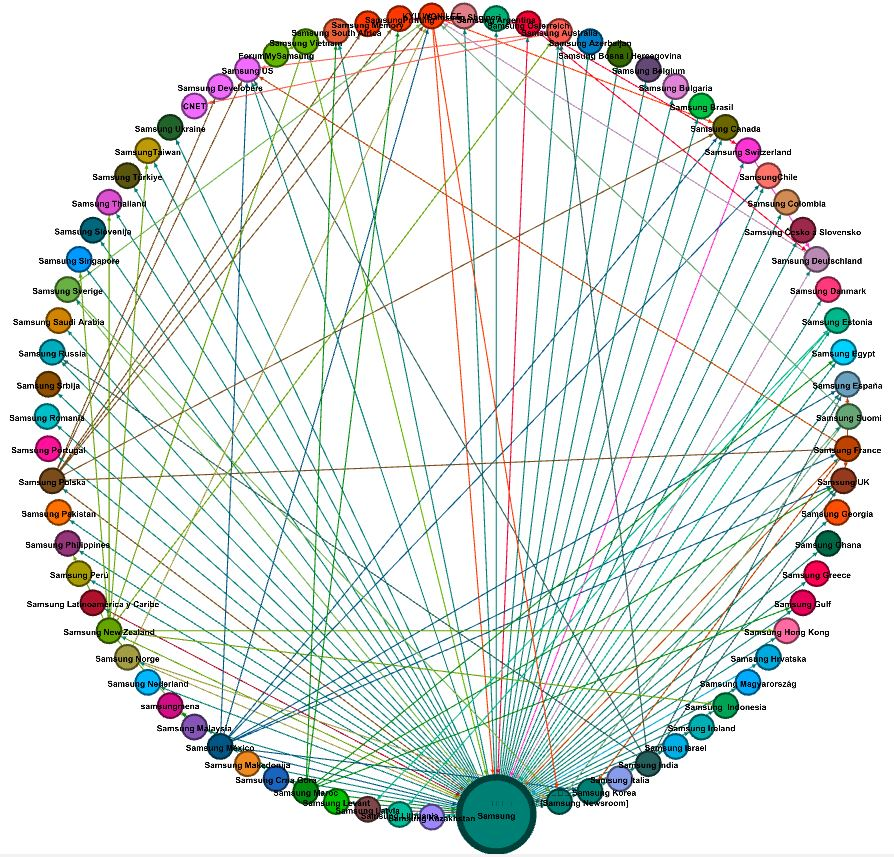
\includegraphics[width=0.8\textwidth]{photos/section3/third_painting.jpg}
		\end{center}
	Απο την πιο πάνω εικόνα μπορούμε εύκολα να παρατηρήσουμε πως ο κεντρικός και ισως ο πιο σηαντικος κόμβος να είναι ο "Samsung" ο οποίος είναι με πράσινο χρώμα. Οι δύο δεξιές θέσεις απο αυτο το κόμβο είναι επίσης με πράσινο χρώμα αφού και αυτοι οι κόμβοι είναι κανάλια απο την ίδια χώρα, την Νότιο Κορέα.
	\label{chap:graphical_representation_3}
	
	
	\section{Βασικά στοιχεία Δικτύου}
	komboi klp(vlepe palies ergasies )
	
	\textcolor{red}{gia na anniksis thn istoria me gephi mpe pou to repo men ksiaseis j na kameis allo(git hub Desktop j anikse file explorer)}
	\label{chap:network_asics_4}
	
\end{document}
